\documentclass[a4paper, 12pt]{report}
\usepackage[utf8]{inputenc}
\usepackage{graphicx}
\usepackage{graphics}
\usepackage[backend=biber,style=alphabetic,]{biblatex}
\usepackage{amsmath}
\usepackage{multicol}
\usepackage{caption}
\captionsetup{
  font=small,
  labelfont=bf,
  tableposition=top
}
\usepackage{hyperref}
\usepackage{indentfirst}
\usepackage[skip=10pt plus1pt]{parskip}
\usepackage[top=0.5in, bottom=0.5in, left=0.5in, right=0.5in]{geometry}
\hypersetup{
    colorlinks=true,
    linkcolor=cyan,
    citecolor=cyan,
    filecolor=magenta,
    urlcolor=cyan,
    pdftitle={Document Image Binarization},
    pdfpagemode=FullScreen,
}

\graphicspath{ {./images} }

\title{
    A Composite Technique for Degraded Document Image Binarization \\[12pt]
    \large
    ITRI617 \\[10pt]
    BSc. Hons. Computer Science and Information Systems
    Prof G. Drevin \\[10pt]
    Computer Science and Information Systems \\[10pt]
    Potchefstroom Campus NWU
}
\author{Johan Venter}

\addbibresource{refs.bib}

\begin{document}

\maketitle
\newpage

\tableofcontents
\newpage
\chapter{Abstract}
\section{English}
Before the digital age, all information was stored as written documents, but in a world overflowing with powerful processing tools, there emanates a need to digitise these documents for analysis, inference, data extraction etc. in a meaningful way. Stored for long periods, historical documents in archives tend to degrade. In this context, document degradation is defined as any artefact on the document that can cause ambiguity in differentiating the content of the document from its background. Therefore, a meaningful solution for a digital copy of a written document would contain only the useful content in the image, rid of the degradation. The process of extracting the textual content from the background and degradation is known as document image binarization~\cite{su2012robust}. The purpose of this project was to secure an understanding of the current state of document image binarization, the techniques and methods used, the obstacles encountered, the efficacy of current methods and finally produce an artefact that demonstrates a solution using information gained from research. The final version of the artefact exists as a composite implementation of existing ideas and methods that were chosen by implementing and comparing various image processing techniques. The program receives a degraded document image as input and transforms it into a binary image.

\section{Afrikaans}
Voor die digitale era is alle inligting as geskrewe dokumente gestoor, maar in 'n wêreld wat oorloop van kragtige verwerkingsinstrumente, ontstaan daar 'n behoefte om hierdie dokumente vir analise, afleiding, data-onttrekking ens op 'n sinvolle wyse te digitaliseer. Geskiedkundige dokumente in argiewe wat vir lang tydperke gestoor word, is geneig om te verneder. In hierdie konteks word dokumentdegradasie gedefinieer as enige artefak op die dokument wat verwarring kan veroorsaak om die inhoud van die dokument van sy agtergrond te onderskei. Daarom sal 'n sinvolle oplossing vir 'n digitale kopie van 'n geskrewe dokument slegs die nuttige inhoud in die beeld bevat, ontslae van die agteruitgang. Die proses om die teksinhoud uit die agtergrond en agteruitgang te onttrek staan bekend as dokumentbeeldbinarisering~\cite{su2012robust}. Die doel van hierdie projek was om 'n begrip te kry van die huidige stand van dokumentbeeldbinarisering, die tegnieke en metodes wat gebruik word, die struikelblokke wat teëgekom word, die doeltreffendheid van huidige metodes en uiteindelik 'n artefak te produseer wat 'n oplossing demonstreer deur gebruik te maak van inligting verkry uit navorsing. Die finale weergawe van die artefak bestaan as 'n saamgestelde implementering van bestaande idees en metodes wat gekies is deur verskeie beeldverwerkingstegnieke te implementeer en te vergelyk. Die program ontvang 'n gedegradeerde dokumentbeeld as invoer en omskep dit in 'n binêre beeld.

\chapter{Introduction}

\section{Project Description}
Document Image Binarization is a field of study concerned with the phase of image pre-processing where a document image is transformed into a bi-level image by separating the text from its background~\cite{su2012robust}. This step precedes the transition to higher-level processing endeavours such as OCR.

\section{Problem Description and Background}
\subsection{Degradation}
There are many obstacles encountered in the process of binarizing historical document images. The main issues are centred around the degradation of written documents. Degradation in this context is seen as a loss of quality that limits the performance of image processing systems~\cite{Baird2007}. In the case of substantially degraded document images, binarization becomes an increasingly difficult task, since the degree and nature of the degradation can be irregular and unpredictable, differing substantially from image to image. Handling document degradation is the most difficult part of image binarization in that there are many categories of degradation that vary substantially in their characteristic qualities. This property makes the development of a model for degradation extremely difficult. Moreover, each image is usually comprised of numerous forms of degradation in different locations with no regular or predictable pattern, and this forms the crux of our problem.

\subsubsection{Natural Environment}
The key issue here is the physical deterioration of the original document. Common traits include blur, varying contrast, smudges and blotches, bleed-through text, variable character intensities and stroke widths, artefacts that cover entire sections of text, non-uniform noise or illumination etc.~\cite{gatos2006adaptive} ~\cite{ait2022innovative}. Although the degradation of a typical document image consists predominantly of the deterioration of the original physical document, each subsequent step in the processing of an image introduces some form of noise and artefacts.

\subsubsection{Scanning Induced}
A scanning device is used to obtain a digital version of an image. Due to unavoidable processes, a whole new range of noises and artefacts are introduced to the digital document. Some corrections are automatically made by the scanning devices, mostly colour corrections such as “gamma correction” which adapts the scanned image to be displayed accurately on a monitor~\cite{smoaca2011id}, but other noise patterns persist, such as noise due to the inevitable material properties of the light sensors used in scanning devices and the way photons are detected or the small imperfections in the sensor’s movements and architecture~\cite{smoaca2011id}. Examples include the scanning of an image that produces reflection artefacts or discrepancies due to an uncalibrated sensor. The quality of the sensor will also affect the resolution of the digital result.\par

After an image has been scanned, it is compressed to an image format like JPEG. Since this is a lossy compression standard, a lot of the original image data is discarded or modified along with other artefacts that are introduced to store the image in a compact format~\cite{eskenazi2016stability}. These changes may be undetectable to the human eye, but is still a loss of original data and will affect the binarization process~\cite{Baird2007}.

\subsection{Methods and Approaches}
Due to the random nature of the image degradations, the development of techniques that accurately model degradations on a wide range of images is met with great difficulty. As such many different approaches have been made towards the advancement of the field and have popularized Image Binarization as a research area~\cite{ait2022innovative} with international competitions such as the recurring DIBCO international competition dedicated to advancing the field. \par

When developing a method that binarizes degraded document images effectively, prior analysis of the document's features plays the most significant role. That requires analysis of the characteristics of the relevant document images and how they differ, as well as how the document content and properties affect the processing method. This leads to a better understanding of the typology and characteristics of these digital documents and how to enhance the desired properties or get rid of unwanted properties. Papers on existing methods proceed on this assumption directly or indirectly. Since our concern is with the binarization of exclusively textual documents and their representation as bi-level images, we can disregard multi-spectral image analysis and focus on monochromatic/grey-level images.

\subsubsection{Global, Local and Adaptive Methods}
From this point, research papers on this topic typically approach the enhancement method of document images using a step-by-step scheme, where each step is a process based on some existing method developed within the context of general image processing that modifies or extracts information from the document image. These methods broadly fall into global or local categories based on how thresholds and enhancements are calculated. Local methods are more adaptive since they calculate statistics of pixels in a neighbourhood around a pixel ~\cite{gatos2006adaptive}. Global methods provide high-level information on the overall characteristics of the image and are less adaptive since it calculates a single parameter using statistics about the entire image that is then used on every pixel~\cite{gatos2006adaptive}. Adaptive methods embrace the benefits of both categories by modifying the image using a combination of global and local statistics. This hybrid approach produces better results on a wider range of degraded documents.

\subsubsection{Scanner Models}
Text Documents are scanned in some way to produce a digital version. Different types of noise are introduced in the scanning process. As indicated by~\cite{smoaca2011id}, the most common noise patterns have been modelled successfully, but as ~\cite{eskenazi2016stability} points out, there are many more unmodelled noise profiles present in scanned document images that aren’t modelled as easily and are mostly modelled empirically.

\subsubsection{Denoising}
Noise is random high-frequency variations in the colour intensities of an image that look like minor disturbances in the context of the entire image. The high-frequency nature of image noise is what denoising methods rely on when attempting to remove it. There is a myriad of different denoising techniques broadly falling into two main categories, spatial filtering and transform domain filtering and each has numerous sub-categories \cite{motwani2004survey}.  Some denoising filters are modelled to remove specific types of noise such as Gaussian noise, Poisson noise, salt and pepper noise etc.

\subsubsection{Contrast Analysis}
Contrast filters identify the areas in an image with high colour intensity disparity or high contrast between neighbouring pixels. This is useful in locating the edges of character strokes. The advantage of using a local contrast or gradient filter such as the one used by~\cite{su2012robust} is that the image intensity levels become normalized, meaning that previously darker or lighter areas in the image now have more similar intensities while retaining the same relative contrast as before. This is a very powerful result since a global thresholding filter can now reliably separate the text and the background without discarding information in previously lighter or darker areas of the document image.

\subsubsection{Thresholding}
Image Binarization is confronted with many obstacles and has some limitations at the moment, such as the need for a robust thresholding method which is an unsolved problem ~\cite{su2012robust}. Thresholding is the common process between each binarization technique. Threshold filters transform an image into a bi-level image, that is, an image with pixels taking on only one of 2 distinct intensity values. This is done by comparing each pixel intensity to a calculated threshold value and setting the new intensity to 0 or 1 depending on the comparison result. Thresholding can also fall into local, global or adaptive categories. Thresholding typically marks the final step before the image enters the post-processing stages.

\subsubsection{Learning Models}
Learning models are used in conjunction with all the previously mentioned categories to aid in parameter estimation and higher-level image modifications. Advanced learning and clustering models are very popular today and are used for denoising, thresholding and character recognition even before the image enters the post-processing stage.

\subsubsection{Post-Processing}
Up to this point, the image has been modified in such a way as to simplify post-processing procedures. Since, at this point, the image is in a bi-level format, higher-level, more complex processing methods can now be used such as Edge and Stroke detection, Stroke width estimates for identifying remaining noise, learning models and OCR.

\subsubsection{Reseach}
This section has outlined the current approaches and challenges related to the field of document image binarization. The scope of this study will entail acquiring a grounded understanding of the specific techniques implemented and their inner workings. Their rationales will be evaluated and compared with others to identify candidate methods. The candidate methods will be implemented and evaluated for the procurement of their respective benefits and drawbacks. This study will aim to deliver a program that is composed of various implementations of the best-performing methods.
\newpage

\section{Aims and Objectives of the Project}
\subsection{Aims}
This study aims to research then collect, develop and adapt a collection of methods and models that can identify and isolate general characteristics of degraded document images. The second goal is to then adapt an existing generic method by integrating these models, which takes a digital document image as input and produces a binarized image that can be used in post-processing endeavours.

\subsection{Objectives}
\begin{itemize}
    \item Aquire an understanding of existing techniques used in image processing and evaluate their rationales.
    \item Compile a collection of candidate techniques and mathematical and statistical models that can best isolate and remove the unwanted artefacts in a degraded document image.
    \item Compile and test different adaptations of the paper by ~\cite{su2012robust} that make use of the previously selected models to arrive at a model.
    \item Implement and optimize the developed model.
    \item Deliver an implementation of the method that successfully separates the textual content from the background of any given input image.
\end{itemize}

\newpage

\section{Procedures and Methods}
\subsection{Paradigmatic Perspective}
\subsubsection{Logical Positivism}
Positivism as a research paradigm is grounded on a proposition about the nature of reality and its properties, and the methods by which information and understanding can be obtained. Positivism departs from the belief that reality is composed of material objects that have properties where statements can be derived about these properties using one’s senses~\cite{putnam2012philosophy}. This idea rests on actual, objective reality, meaning that objects exist absolutely and independently of the perceiver. Reality can therefore be described in terms of constant universal properties, presentable as perceivable truths. Positivism takes reality as a collection of interdependent objects governed by laws and symmetries that conduct all occurring events. As assumed by determinism, observed events are dependent on other factors and an understanding of the relevant factors allows the prediction and control of events~\cite{kivunja2017understanding}.\par

Positivism assumes that everything knowable can be discovered. The paradigm introduces the methods by which these truths can be obtained. Facts can be empirically collected or derived by using the scientific method. The scientific method entails the use of logical reasoning, deduction, the formulation of hypotheses, experimentation and mathematical methods to derive conclusions, therefore, creating an understanding of a part of reality~\cite{kivunja2017understanding}.

\subsubsection{Application}
This research paradigm is well suited for this study since it relies on the acquisition of material text documents that have certain characteristics. These characteristics include the textual content of the documents as well as the associated artefacts.\par

The proposition of objectivity is appropriate in this context since the text on a document consists of characters that can each be designated a ubiquitous category. That is, the method assumes the use of a document with textual content that will be transformed into an image containing the same objective textual content. The product of the method is an artefact delivering a distinct separation between text and background, implying that the ideal solution produces an image containing only the textual content of the original image. The performance of this artefact will consequently be evaluated by empirical methods.\par

Unwanted artefacts and degradation can therefore be viewed deterministically i.e., there are external factors that produce these artefacts and an understanding of them can be used to shape empirical models. By using scientific methods such as mathematical and statistical analysis, empirical modelling and experimentation one can analyse the documents and model their properties and dependent factors.


\subsubsection{Methods}
This study will start with research on digitised document images i.e., the associated processes in creating them and their artefacts as well as insight into the properties and characteristics that distinguish them from other types of scanned images. The resulting context will be used to explore existing document image binarization solutions and the challenges they encounter. The existing solutions will then be decomposed into their distinct components, that is, broken down into the individual parts of the process, that can each be described by the specific goal it aims to achieve. These techniques will undergo experimental analysis to compare their results. Resulting inference on these results will be used in the development of an artefact that will demonstrate an implementation of the chosen methods. \newpage

\section{Project Management and Plan}
\subsection{Plan}
\subsection{Scope}
The research of this project will be confined to the binarization of textual document images only. The textual content of the documents can be either typed or written text. This study will focus on a wide range of degraded images. The resulting artefact will aim to take a degraded document image as input and deliver a modified bi-level image rid of all degradations yet containing the same text as the original image. Since the artefact will produce a bi-level image, research on the nuances regarding colour and multi-spectral processing and analysis will be omitted. Using the paper by~\cite{su2012robust}, the study will compose an adaptation of their technique as an artefact.

\subsection{Limitations}
The topic of document image binarization is a well-established field with numerous years of relevant research. This means that due to time constraints and research background, this study cannot be comprehensive at that scale.
Due to the nature of the degradation of the documents as well as other previously mentioned factors, there are some trade-offs involved in removing these defects that result in either a loss of important information or the persistence of prominent degradations. This study is primarily concerned with existing techniques with a secondary objective of novel development in the field.

\subsection{Risks}
As of the time when this was written, no risks were identified in conducting this study or the development of the artefact since it makes use of open-source libraries and datasets and does not collect any personal information from anyone. The results of this project are also risk-free since it dabbles in a well-researched area.

\section{Development Platform, Resources and Environments}
The chosen models and methods will be implemented as an independent script within the python programming language since it is a language optimised for prototyping and it is a simple language but most importantly, it provides substantial support, environments and libraries for image processing. The open source python libraries that will be used are:
\begin{itemize}
    \item \href{https://numpy.org/}{numpy}~\cite{numpy}
    \item \href{https://scikit-image.org/}{scikit-image}~\cite{scikit-image}
    \item \href{https://scikit-image.org/}{scipy}~\cite{2020SciPy-NMeth}
\end{itemize}

A simple front-end application will be constructed using the \href{https://angular.io/}{Angular Web Framework}~\cite{angular_2022} for displaying the input and output images and navigating between them for demonstration as well as development and testing. The front-end application will retrieve the results from the python script through a locally hosted \href{https://nodejs.org/en/}{Nodejs}~\cite{nodejs_2022} server that will execute the package on the chosen image since it is a simple reliable way of serving images and results. The implementation of the models in python will not depend on any of the auxiliary architectures. \par

The images chosen for testing and demonstrations are provided by \href{https://vc.ee.duth.gr/h-dibco2016/}{DIBCO 2016 Handwritten DocumentDataset}. They were chosen since they are open-source, and therefore free from legal implications (within regulation). These datasets are also the ones used by the yearly \href{https://dib.cin.ufpe.br/#!/resources/dibco}{DIBCO} competition.

\section{Ethical and Legal Implications and Dealing with These}
see addendum A

\chapter{Literature Review}
This section will discuss the ideas and challenges surrounding the binarization of degraded document images. After discussing the image processing pipeline, the first subsection discusses what degradation is, what its causes are, how modelling is approached and lastly presents some current models.

\section{Image Processing Pipeline}
Image binarization falls into the pre-processing stage where degradation and defects are compensated for. The pre-processing stage forms a pipeline of processes that each modify its input before passing it to the next process in the pipeline. The first of these is called the pre-processing stage where degradation and defects are compensated for~\cite{ramanath2005color}. Since this project is concerned with document images, the binarization of the document also falls into the pre-processing stage.\par

As document image binarization aims to separate the textual content from the background by removing degradations, the first question arises: What does degradation on an image look like and how does one model it?

\section{Document Image Degradation}
Degradations or defects on a document image refer to any properties of actual document images that deviate from what can be considered the ideal image that reduces the efficiency of image processing systems~\cite{Baird2007}. When paper documents are printed, copied, faxed and scanned, the documents degrade. Even if it seems insignificant to the human eye, this quality loss can reduce the accuracy of even the most cutting-edge text recognition systems (OCR). Additionally, there is mounting evidence that the quantity and representativeness of training sets as well as the feature selection have a considerable impact on the accuracy of stubborn picture pattern recognition tasks~\cite{Baird2007}. Therefore, the performance of these algorithms hinges on the quality of the binarization result. \par

\subsection{Operational Degradation}
This type of degradation involves the defects produced by the equipment used in obtaining a digital copy of a given document image. An image is converted to digital form using a scanning device. Unavoidable procedures result in the introduction of a wide variety of noise and artefacts into the digital document. Other noise patterns persist, such as the small imperfections in the sensor's movements and architecture. Some corrections are automatically made by the scanning devices. These corrections are mostly colour corrections, such as "gamma correction," which adapts the scanned image to be displayed accurately on a monitor~\cite{smoaca2011id}. Examples include the scanning of an image that produces reflection artefacts or discrepancies due to an uncalibrated sensor. The quality of the sensor will also affect the resolution of the digital result. Since this type of degradation is caused by the scanner, it tends to be easier to model since it is independent of the image and by analysing the effects of the scanner on different images, one can model the defects of the scanner.\par

An image is compressed into an image format like JPEG after it has been scanned. Since this is a lossy compression standard, a significant portion of the original image data is lost or altered~\cite{eskenazi2016stability}. \par

\subsection{External Degradation}
The physical deterioration of the original document is the main problem in this situation. Examples of this type of degradation include blur, fluctuating contrast, smudges and blotches, bleed-through text, variable character intensities and stroke widths, artefacts that cover entire areas of text, non-uniform noise or illumination, etc.~\cite{gatos2006adaptive} ~\cite{ait2022innovative}. This type of degradation refers to the defects related to the physical state of the document, independent from the result produced by the apparatus used to scan the document. This category of degradation can be the most difficult to model as it cannot be generalized since different degradations can appear at different intensities at various locations in the document image. This can be further illustrated by the fact that these types of degradation sometimes overlap with what is not considered degradation. As an example, a model that may be good at identifying and removing ink-smearing may compromise the quality of the document in areas where ink-smearing is not present.

\subsection{Inevitable Disparities}
This type of degradation is described by the inevitable physical properties of light, reflection, and the way that scanning devices scan images as well as properties like the resolution of the images. Some of these degradations must be modelled and analysed statistically~\cite{Baird2007}, but for some defects, there are no existing models and are considered roadblocks in the image pre-processing pipeline.


\section{Issues With Modelling}
\cite{Baird2007} notes that the main components affecting the modelling process are:
\begin{itemize}
    \item \textbf{Parameterization}: The observed degradation must be able to be described by a fixed set of numerical parameters. Otherwise, the model is of no use.
    \item \textbf{Randomization}: If the degradation is modelled as having properties that behave in a probabilistic manner, their distributions should be parameterized in the model.
    \item \textbf{Validation}: Since some of the model parameters will inevitably be probabilistic, one needs to compensate for this by accounting for certain margins of error.
    \item \textbf{Parameter Estimation}: Once the model is developed, a distribution fitting the real distribution can be generated by tuning the parameters.
    \item \textbf{Correlation}: When modelling using statistics and probability distributions, one can easily mistake correlation for causation, therefore the model must be thoroughly evaluated by predicting the output of changes in parameters and verifying those predictions. Unexpected results may indicate that the model is incomplete.
\end{itemize}

\section{Modelling}
Document image degradation can be modelled in two main ways. The first is to analyse and model the physical properties of the factors that cause these defects. This can in turn deliver a degradation model based on the workings of the environment that the images are subjected to. Although this method will theoretically yield the most accurate, reliable results, this approach can quickly become overcomplicated as~\cite{Baird2007} points out. The second approach is to model the degradation empirically. This involves developing a model that can replicate the effects of the degradation, disregarding the cause. The main way this is done is by using statistical analysis. Of course, these methods can be combined to form a hybrid model.

\subsection{Noise}
The devices used to scan documents introduce various forms of noise to the document. Some elementary models include Gaussian noise, Rayleigh noise, Gamma noise, Exponential noise, Uniform noise, and Salt-and-Pepper noise each having a probability density function that describes the distribution of the noise in an image~\cite{gonzalez_woods_pearson_hall}. Since this topic has been the subject of research for a significant amount of time (more than 80 years), existing noise models are very sophisticated and although most models are statistics based, the papers also consider the underlying physical structure of the scanning device in their models such as the scanner model depicted by~\cite{gou2007robust} or the range of noise patterns by imaging sensors modelled by~\cite{lukas2006digital}.\par

Research on image denoising is extensive but can firstly be classified according to which domain the noise is filtered in. Noise removal can either be done in the spatial domain or in the frequency domain. Images must undergo the Fourier Transform to map them onto the frequency domain. In spatial domain filtering there exist some popular methods such as Mean, Wiener and median filtering. Filtering in the frequency domain yields many more opportunities such as filtering in the wavelet domain using linear, non-linear, and other models.


% ~\cite{gatos2006adaptive} use a low-pass Wiener filter as a first procedure to denoise the image. The Wiener filter produces a noise-reduced image based on the minimum square error measure. The Wiener filter removes background noise effectively but blurs the image significantly. Other noise filtering methods such as Median filters or wavelet domain filters are also popular.





\chapter{Description of the Artefact}
The development of this artefact was inspired by the method used by~\cite{su2012robust} for document image binarization. Document Image Binarization, in this context, is a field of study within the phase of image pre-processing where a digital version of a written document is transformed into a binary image, separating the text from the noise, degradation and background~\cite{su2012robust}. Therefore, this artefact had a clear objective, namely, to obtain a digital written document, process the image by removing unwanted artefacts and deliver a binary image containing only the text from the original image.\par

This artefact, therefore, is a program written in python that receives a document image as input and then passes the image through a pipeline of distinct processes, each modifying the image or extracting information about the image for use in the following process. The resulting program uses three main libraries namely \href{https://numpy.org/}{numpy}~\cite{numpy}, \href{https://scikit-image.org/}{scikit-image}~\cite{scikit-image} and \href{https://scikit-image.org/}{scipy}~\cite{2020SciPy-NMeth} in conjunction with custom-developed methods to compose the processes that make up the pipeline. \par

A document image is provided as input and is converted to a grayscale image for processing. This is done by averaging the colour channels of the image into a single channel. It is then passed through a series of steps that each modify it in some way. The process is comprised of four main steps. The images used for testing and
demonstrations are open-source, provided by \href{https://vc.ee.duth.gr/h-dibco2016/}{DIBCO 2016 Handwritten DocumentDataset}.

\noindent
\begin{minipage}{\linewidth}
    \centering
    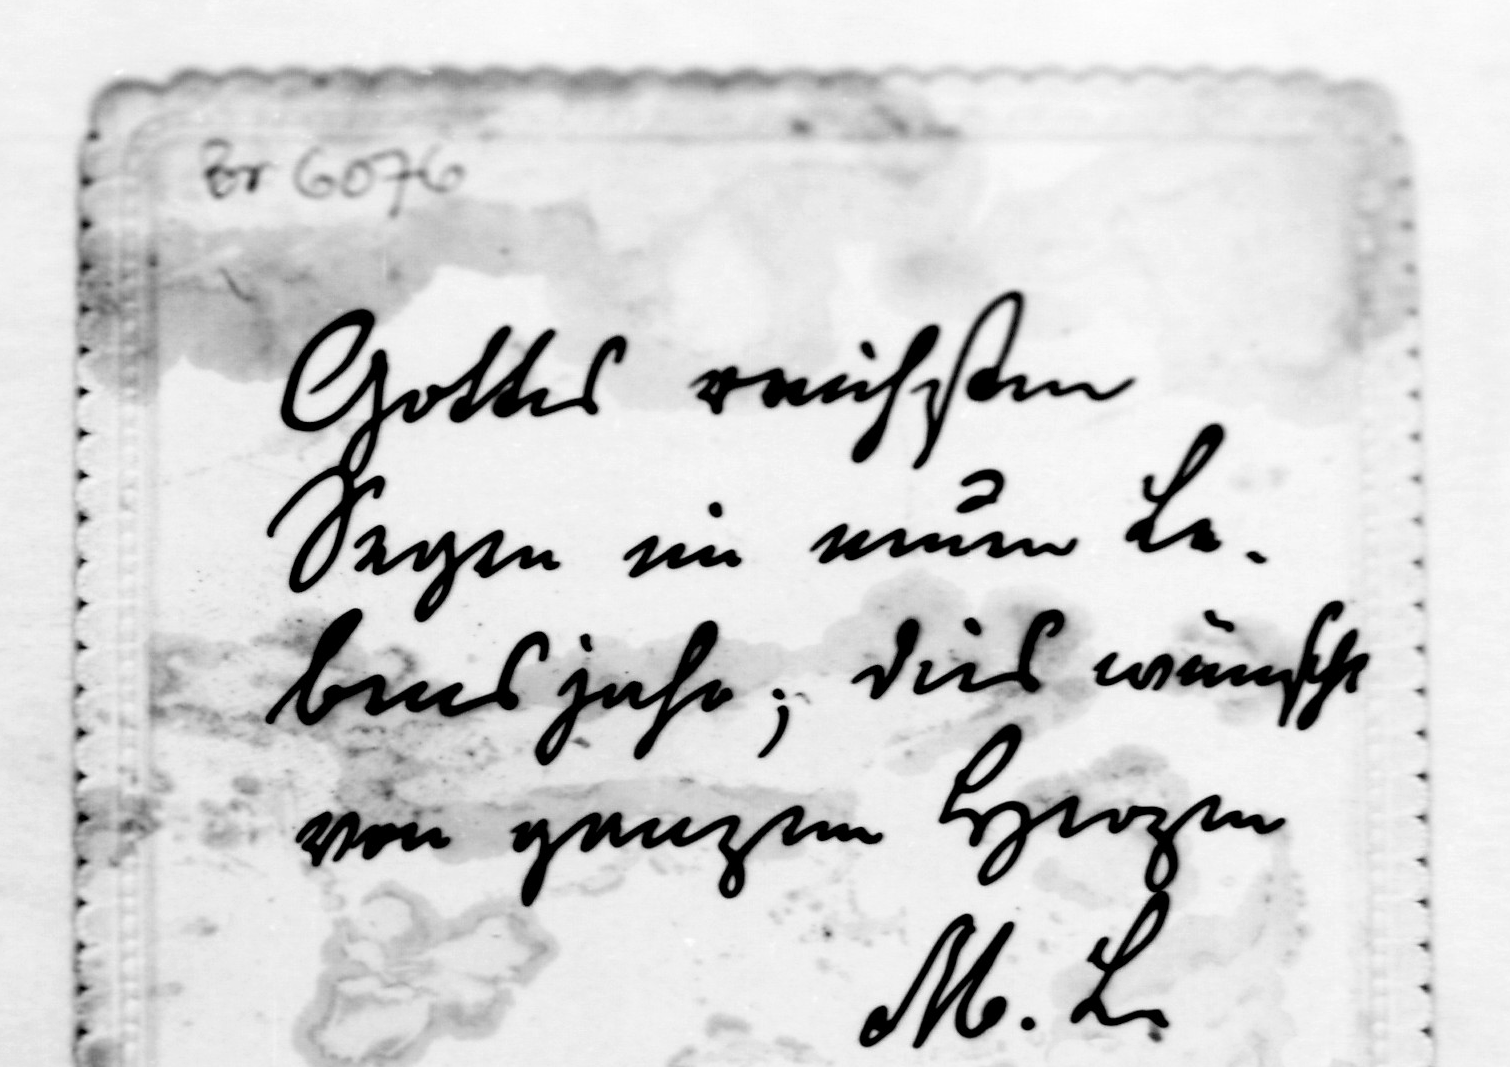
\includegraphics[width=8cm]{original.png}
    \captionof{figure}{Original Document Image}
    \label{fig:1}
\end{minipage}

\subsection{Denoising}
After the image is converted to grayscale, the image is denoised. Both low and high-frequency noise is prevalent in most images. The low-frequency noise or coarse noise is filtered by applying the wavelet denoising filter available in the scikit-image library. This filter uses the standard deviation of the intensity values of the image as an input parameter as demonstrated in Figure~\ref{fig:2}.

\noindent
\begin{minipage}{\linewidth}
    \centering
    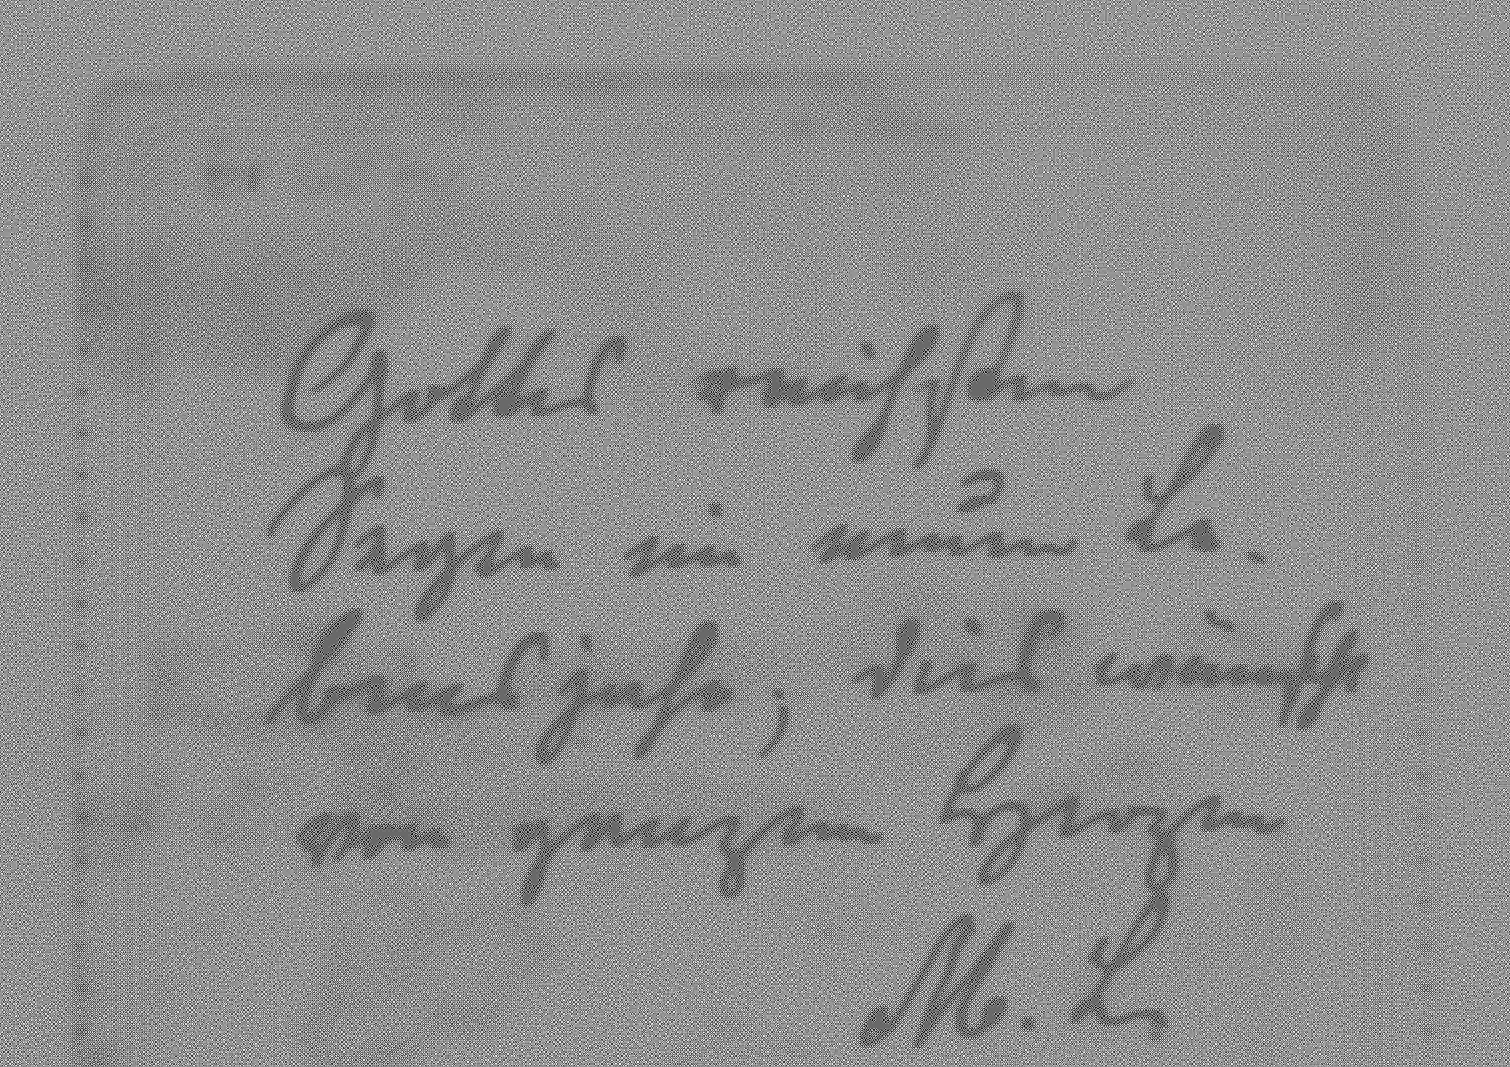
\includegraphics[width=8cm]{wavelet difference.png}
    \captionof{figure}{Noise removed by wavelet filter}
    \label{fig:2}
\end{minipage}

This is followed by applying a custom adaptive wiener filter that uses a 3x3 gaussian kernel to remove low-frequency gaussian noise (Figure~\ref{fig:3}). Note, at this point, that the image's grey-level intensity values cover a vast range.

\noindent
\begin{minipage}{\linewidth}
    \centering
    
\includegraphics[width=8cm]{wiener difference.png}
    \captionof{figure}{Noise removed by wavelet filter}
    \label{fig:3}
\end{minipage}

\subsection{Thresholding}
Otsu's thresholding method is used to convert the denoised image into a binary image by using .

\noindent
\begin{minipage}{\linewidth}
    \centering
    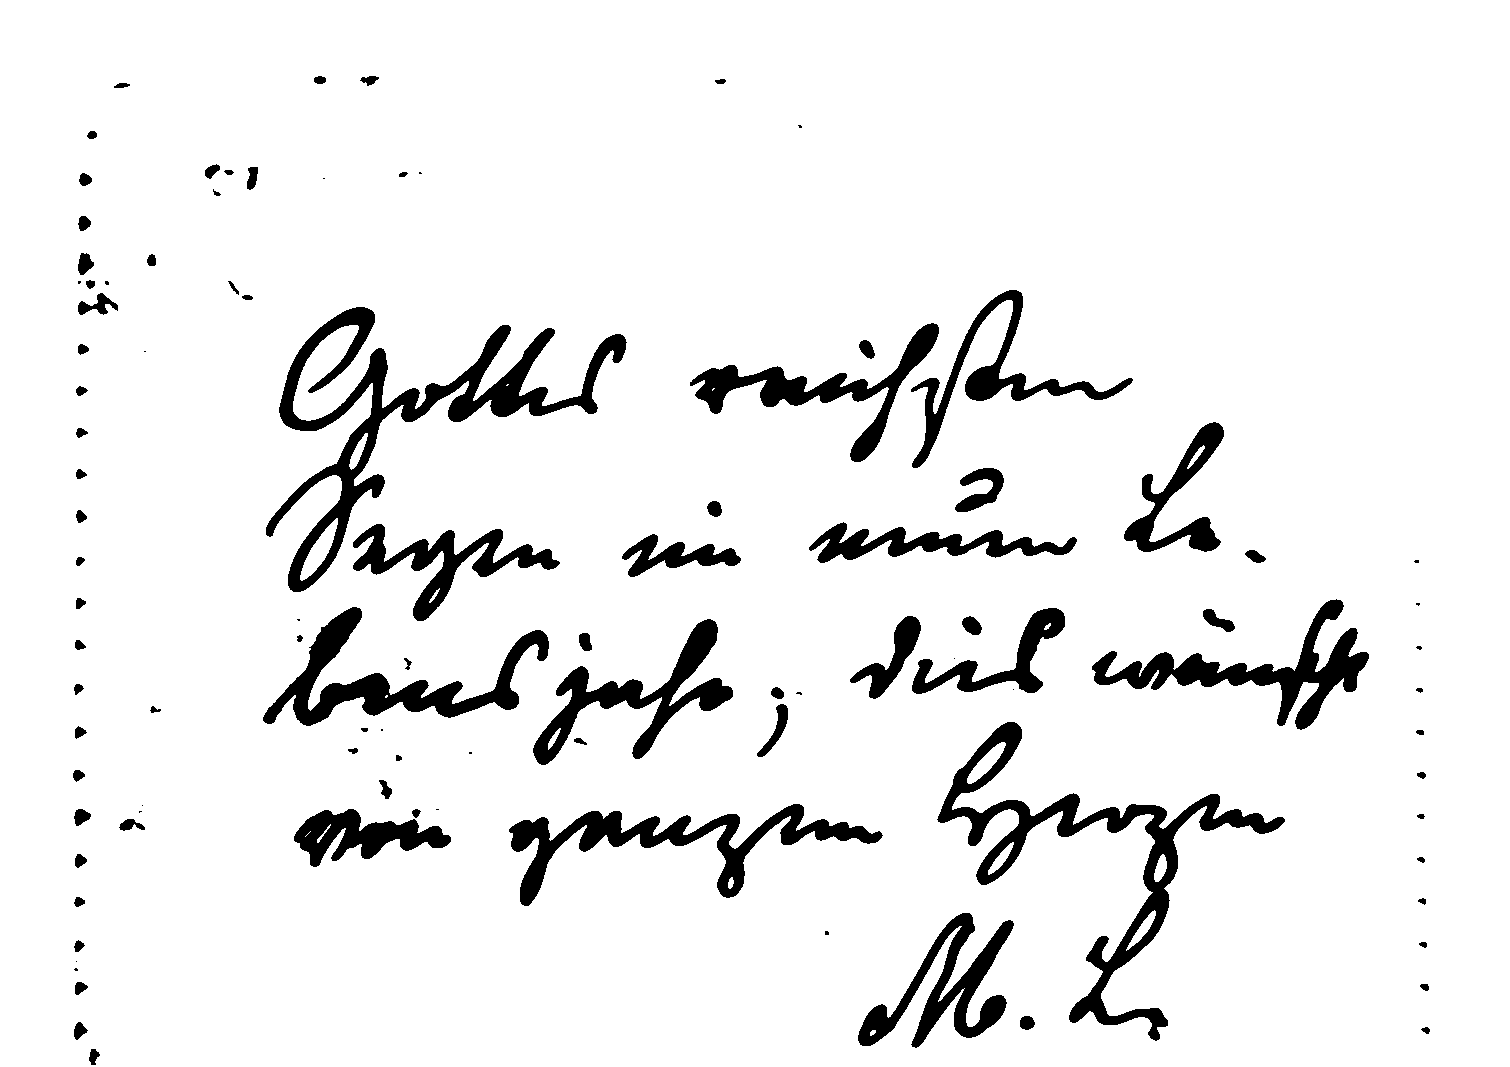
\includegraphics[width=8cm]{otsu thresholded.png}
    \captionof{figure}{Otsu thresholded image}
    \label{fig:4}
\end{minipage}

\subsection{Text Stroke Width Estimate}
An estimation of text stroke width will be utilised in the final step. An effective method of doing this as introduced by~\cite{strokewidth} consists of two main steps, namely performing a distance transform and skeletonizing the image.

\subsubsection{Distance Transform}
The distance transform uses the thresholded image and assigns each pixel a value according to its euclidean distance to the closest white pixel (background pixel), thereby creating an image with the brightest pixels in the centre of the text.

\noindent
\begin{minipage}{\linewidth}
    \centering
    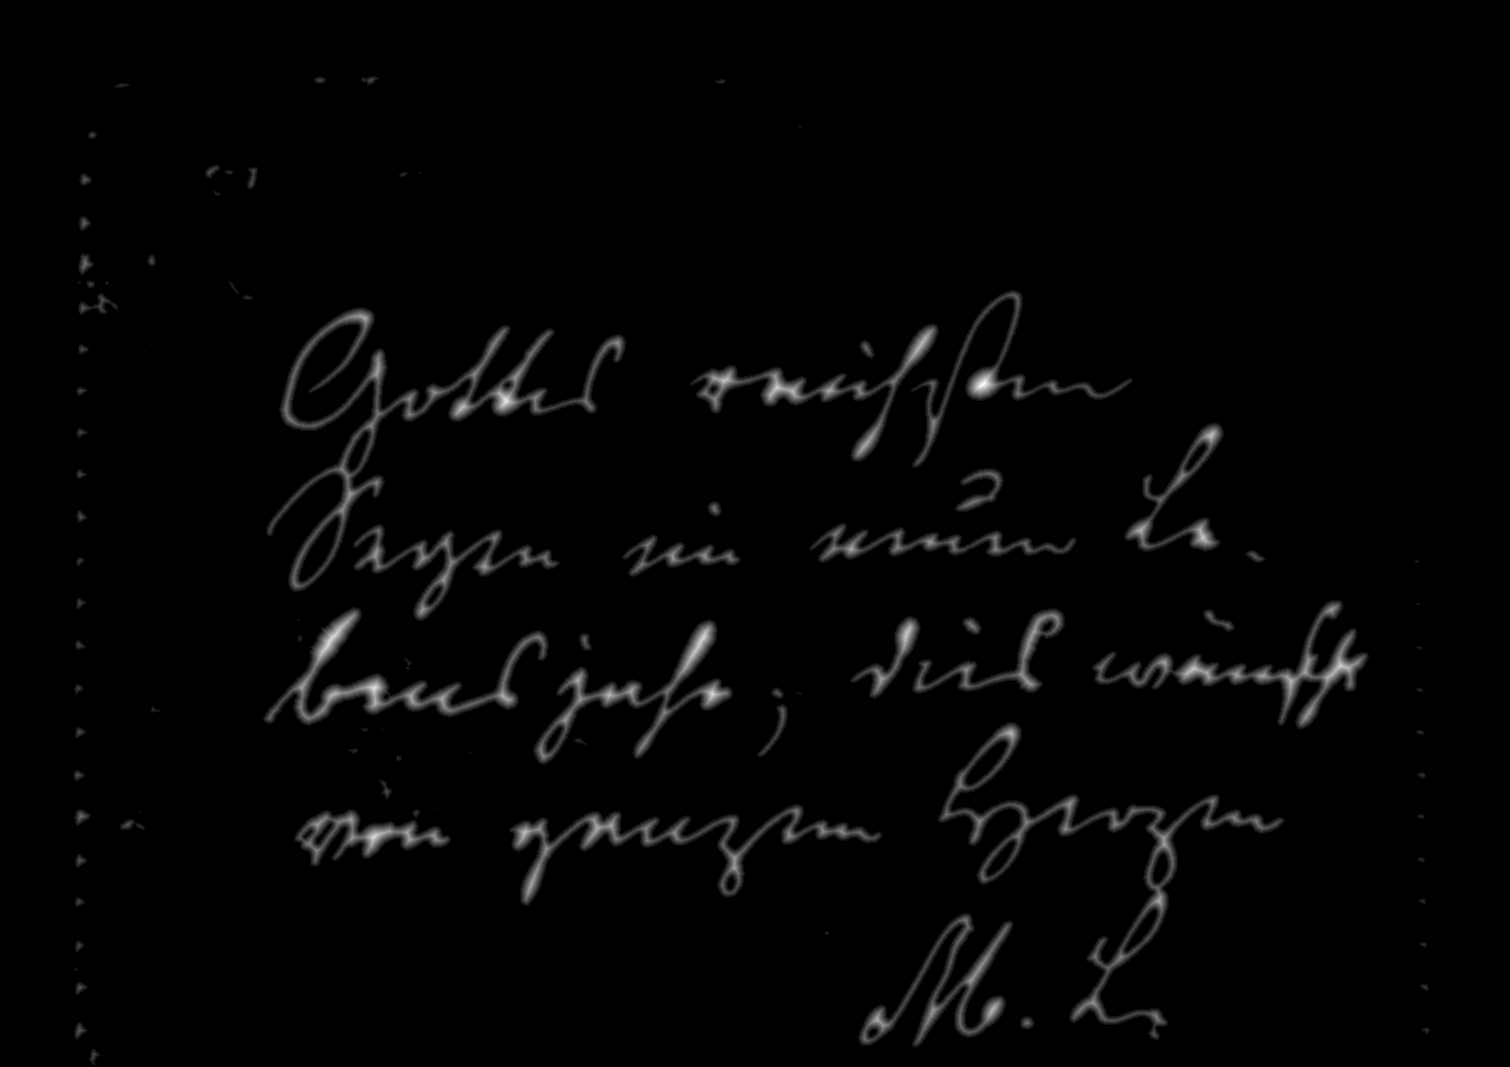
\includegraphics[width=8cm]{distance transform.png}
    \captionof{figure}{Distance transform}
    \label{fig:5}
\end{minipage}

\subsubsection{Skeletonizing}
Skeletonizing an image consists of making multiple passes over an image and detecting the edge pixels. These edge pixels are then removed unless they break the connectivity of the identified object~\cite{scikit-image}.

\noindent
\begin{minipage}{\linewidth}
    \centering
    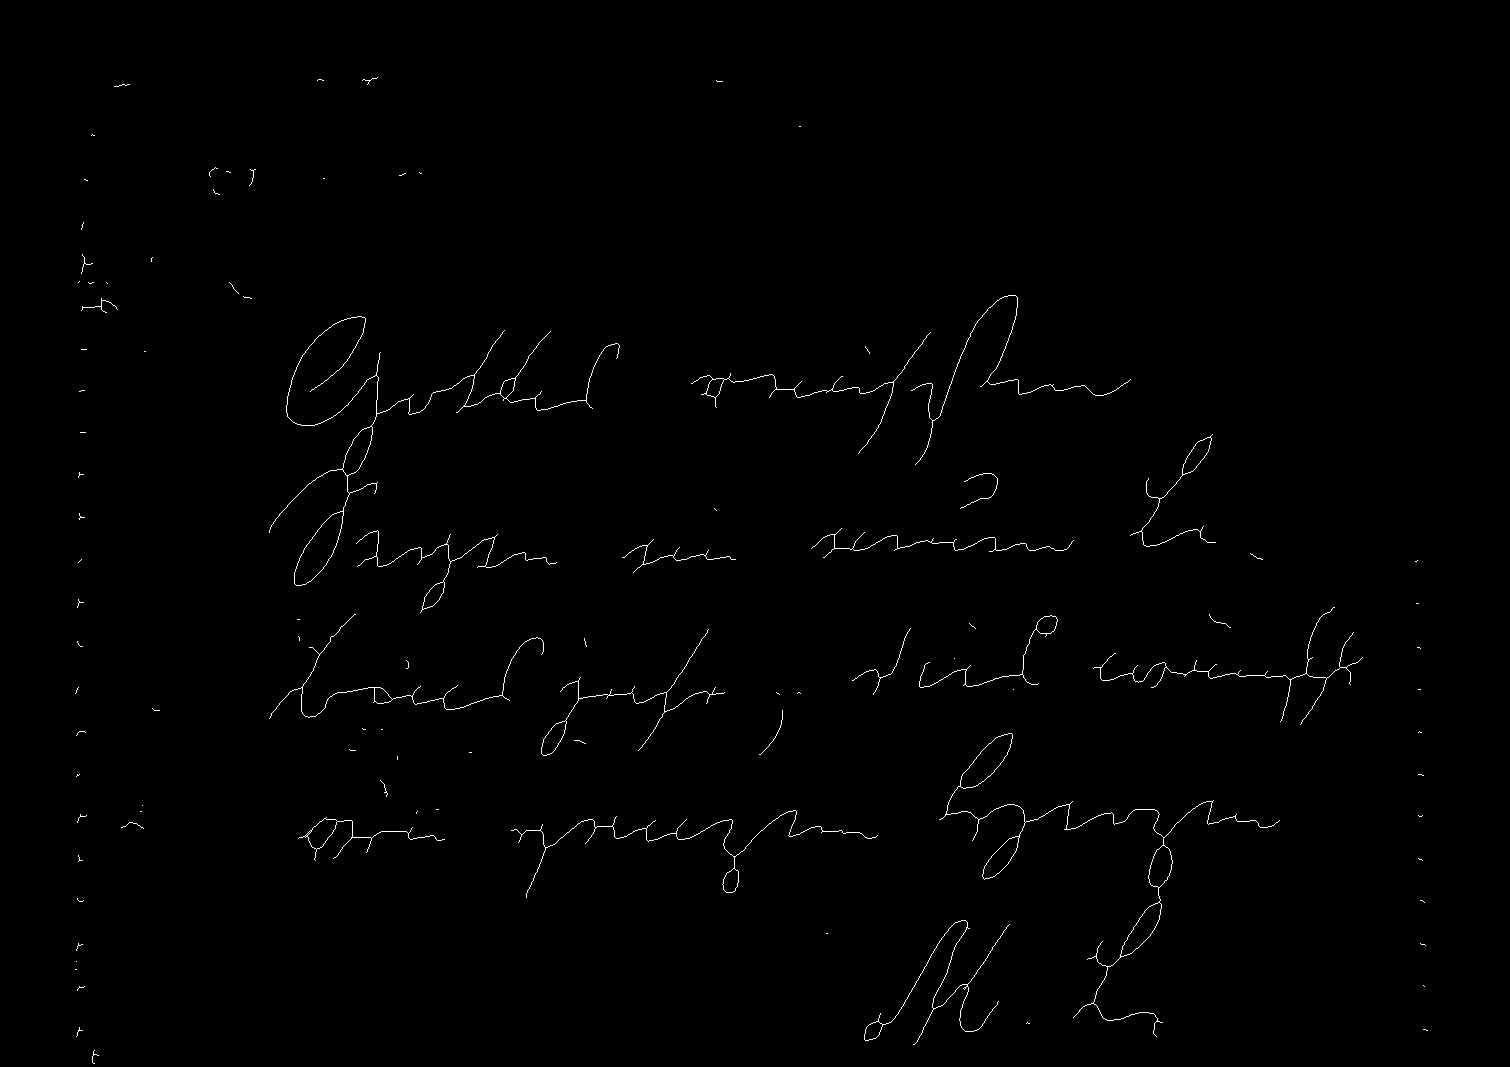
\includegraphics[width=8cm]{skeletonized.png}
    \captionof{figure}{Skeletonizing transform}
    \label{fig:6}
\end{minipage}

The bright pixels in the skeletonized image are then used as indexes for the selection of pixels in the distance-transformed image. The selected pixel values in the distance-transformed image are summed, and averaged to obtain a quantity half of the actual average text stroke width.

\subsection{Median Filter}
Finally, A median filter that uses the calculated stroke width as a parameter passes over the image to remove artefacts on the image smaller than the text stroke to produce the final result.

\noindent
\begin{minipage}{\linewidth}
    \centering
    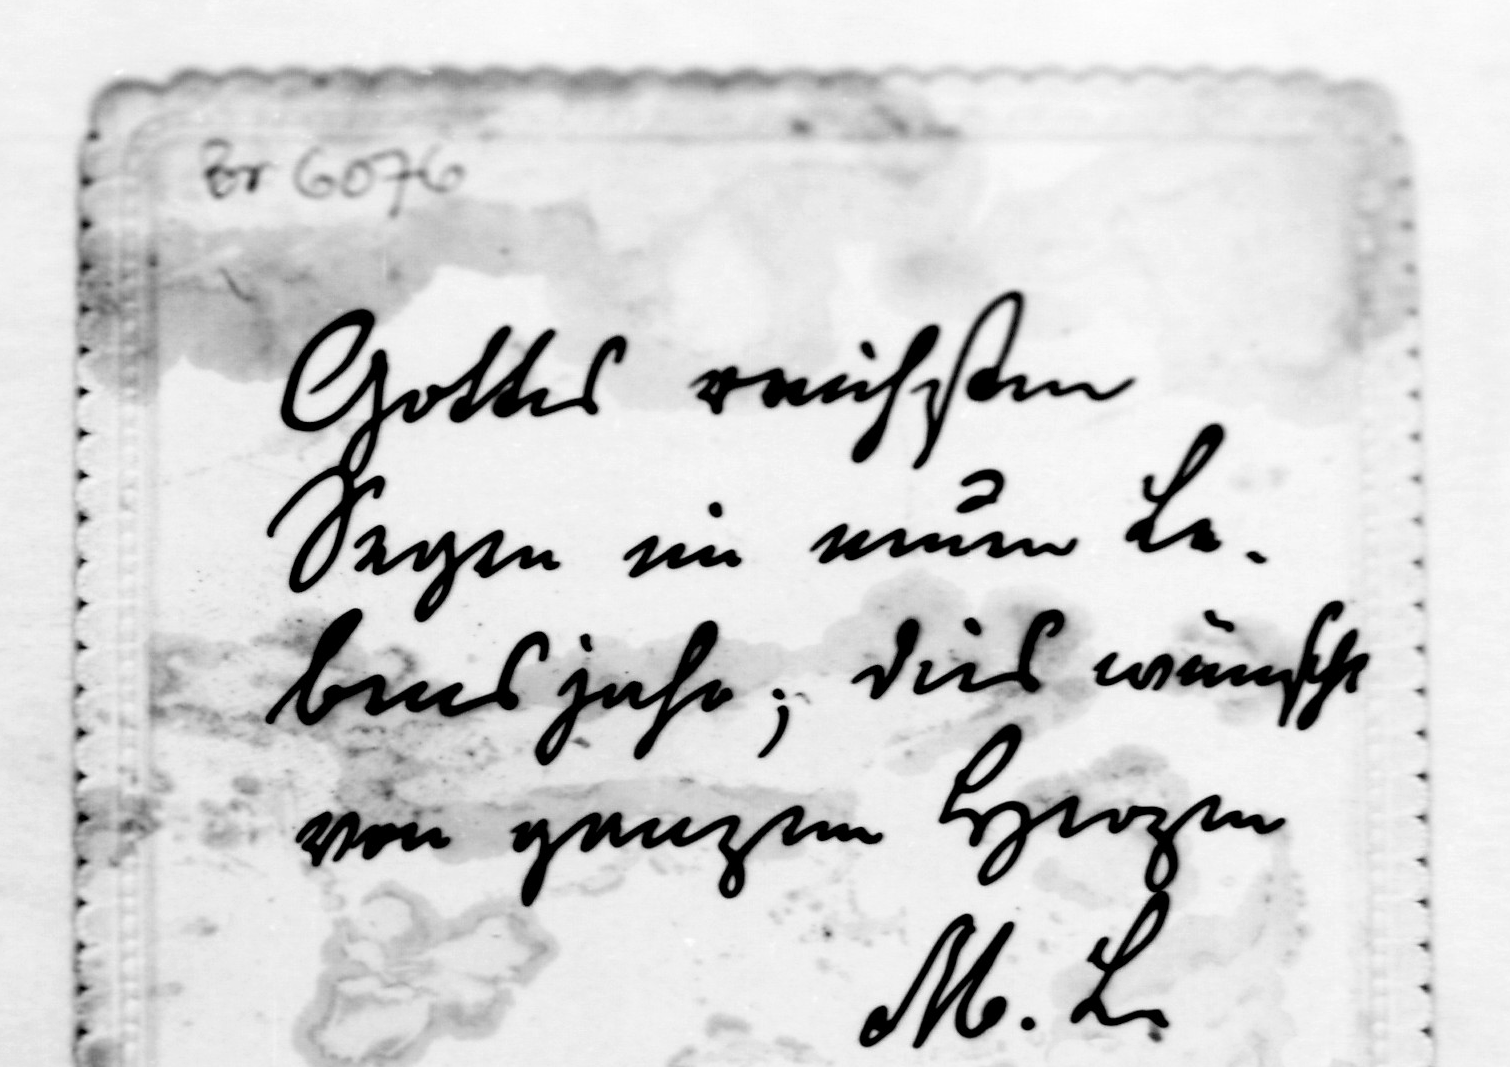
\includegraphics[width=8cm]{original.png}
    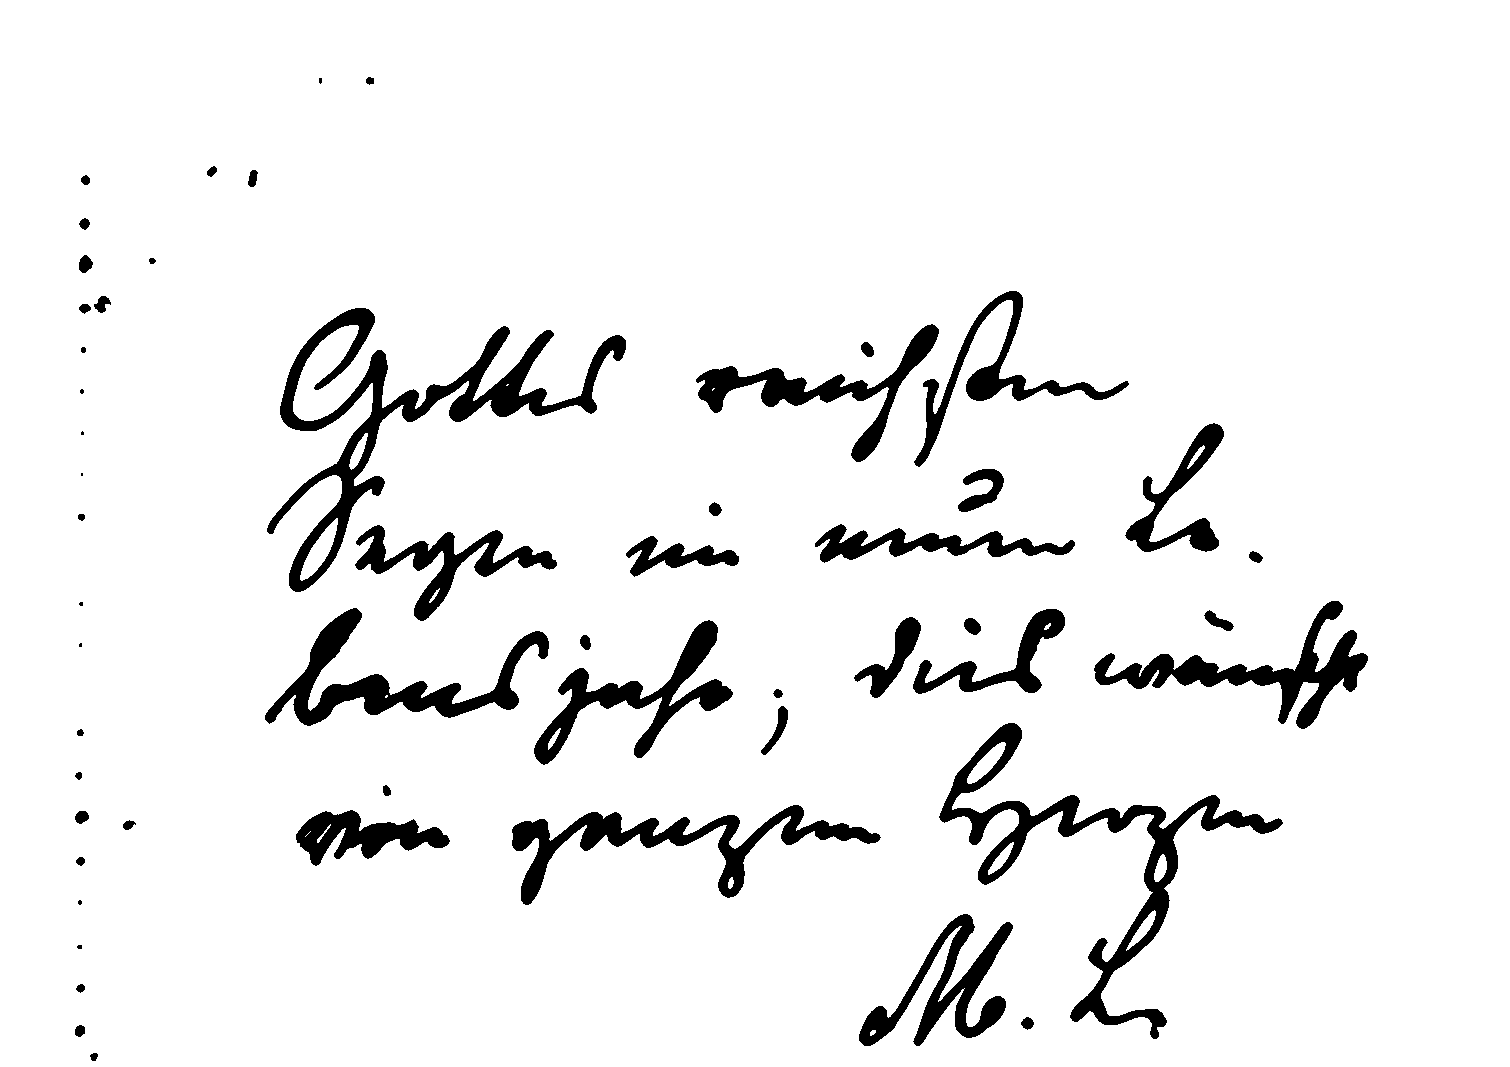
\includegraphics[width=8cm]{output.png}
    \captionof{figure}{Original vs Final Binarized Image}
    \label{fig:7}
\end{minipage}

\newpage

\section{Development Lifecycle}
The general lifecycle of the development of this project involved the iterative research and testing of multiple existing strategies.

\subsection{Research}
The first step in the lifecycle was the research for this project. The research needed to be directed towards gaining an understanding of the problem, the related fields and key terms and jargon related to the problems encountered.

\subsection{Existing Solutions}
Once a firm understanding of the field was established, existing solutions were researched and evaluated. This also required an understanding of the surrounding technologies and fundamentals of the methods used.

\subsection{Development}
Candidate methods, ideas and technoloies were identified and appropriate open source libraries were leveraged where needed. Several methods were implemented, tested and relinquished.

\subsection{Iterative Approach}
Although the main lifecycle of the development of the project was sequential, each step happened iteratively.

% \section{Development of the Artefact}
% As a guide for methods relating specifically to document image binarization, two main sources were utilised~\cite{su2012robust}~\cite{gatos2006adaptive}. For general image processing principles and practices \href{https://numpy.org/}{numpy}~\cite{numpy},
% \href{https://scikit-image.org/}{scikit-image}~\cite{scikit-image} and
% \href{https://scikit-image.org/}{scipy}~\cite{2020SciPy-NMeth} were invaluable.

\subsection{Denoising}
\subsubsection{Wiener Filter}
The Wiener filter is optimal by the mean squared error measure, since it is defined by it. This property along with popular use and consistency of results by ~\cite{6524379}, ~\cite{gatos2006adaptive} makes the wiener filter as well as wavelet filters the obvious choice as candidates for denoising the document images.
\par
~\cite{gatos2006adaptive} describes the use of an adaptive wiener filter that makes use of the local properties in an image to reduce noise using the following formula:
\[I(x,y)=\mu+\frac{(\sigma^2-v^2)(I_{source}-\mu)}{\sigma^2}\]
where \(\mu\) is the local mean, \(\sigma^2\) the variance in a 3 x 3 window and \(v^2\) is the average variance.
\par
The selected algorithm is a variation on the original Wiener filter, called the Wiener-Hunt filter that transforms the image into the freqency domain first by using the fourier transform
\[\hat x = F^\dagger (|\Lambda_H|^2 + \lambda |\Lambda_D|^2)
    \Lambda_H^\dagger F y\]
with \(F\) and \(F^\dagger\) the Fourier and inverse Fourier transforms respectively, \(\Lambda_H\) the Fourier transform of the transfer function and \(\lambda\) a damping constant as described by~\cite{scikit-image}.

\subsubsection{Wavelet Filter}
The wavelet transform decomposes the image into a collection of wavelets. A wavelet is a wave-like function, that has a finite 'energy' and symmetric area around the x-axis. The transform can be interpreted as the convolution of a set of wavelets over the image that will output a signal proportional to the similarity between the wavelets and the image.
\[ \int_{-\infty}^{\infty} f(x,y) \cdot g(x,y) \,dx \]

\par
Other Denoising methods were considered such as total variation denoising and bilateral denoising.

\subsection{Thresholding}

% \subsection{Gradient Image}
% An image is constructed using a formula for identifying local image contrast:
% \begin{equation}
%     \label{E:1}
%     C(i,j)=\frac{I_{max}(i,j)-I_{min}(i,j)}{I_{max}(i,j)+I_{min}(i,j)+\epsilon}
% \end{equation}
% where \(\epsilon\) is a positive infinitesimal. The denominator scales the input according to the local range of values, thereby normalizing the contrast across the image~\cite{su2012robust}. Next, a constant \(a\) is calculated:
% \begin{equation}
%     \label{E:2}
%     a=(\frac{\sigma}{128})^\gamma, \; \gamma \geq 0
% \end{equation}
% \(\sigma\) is the standard deviation of the entire document image intensities.
% By combining \ref{E:1} and \ref{E:2} we derive the final equation they use to construct the Gradient image:
% \begin{equation}
%     \label{E:3}
%     C_a(i,j)=a\times C(i,j)+(1-a)(I_{max}(i,j)-I_{min}(i,j))
% \end{equation}
% Which results in
% \begin{figure}[htp]
%     \centering
%     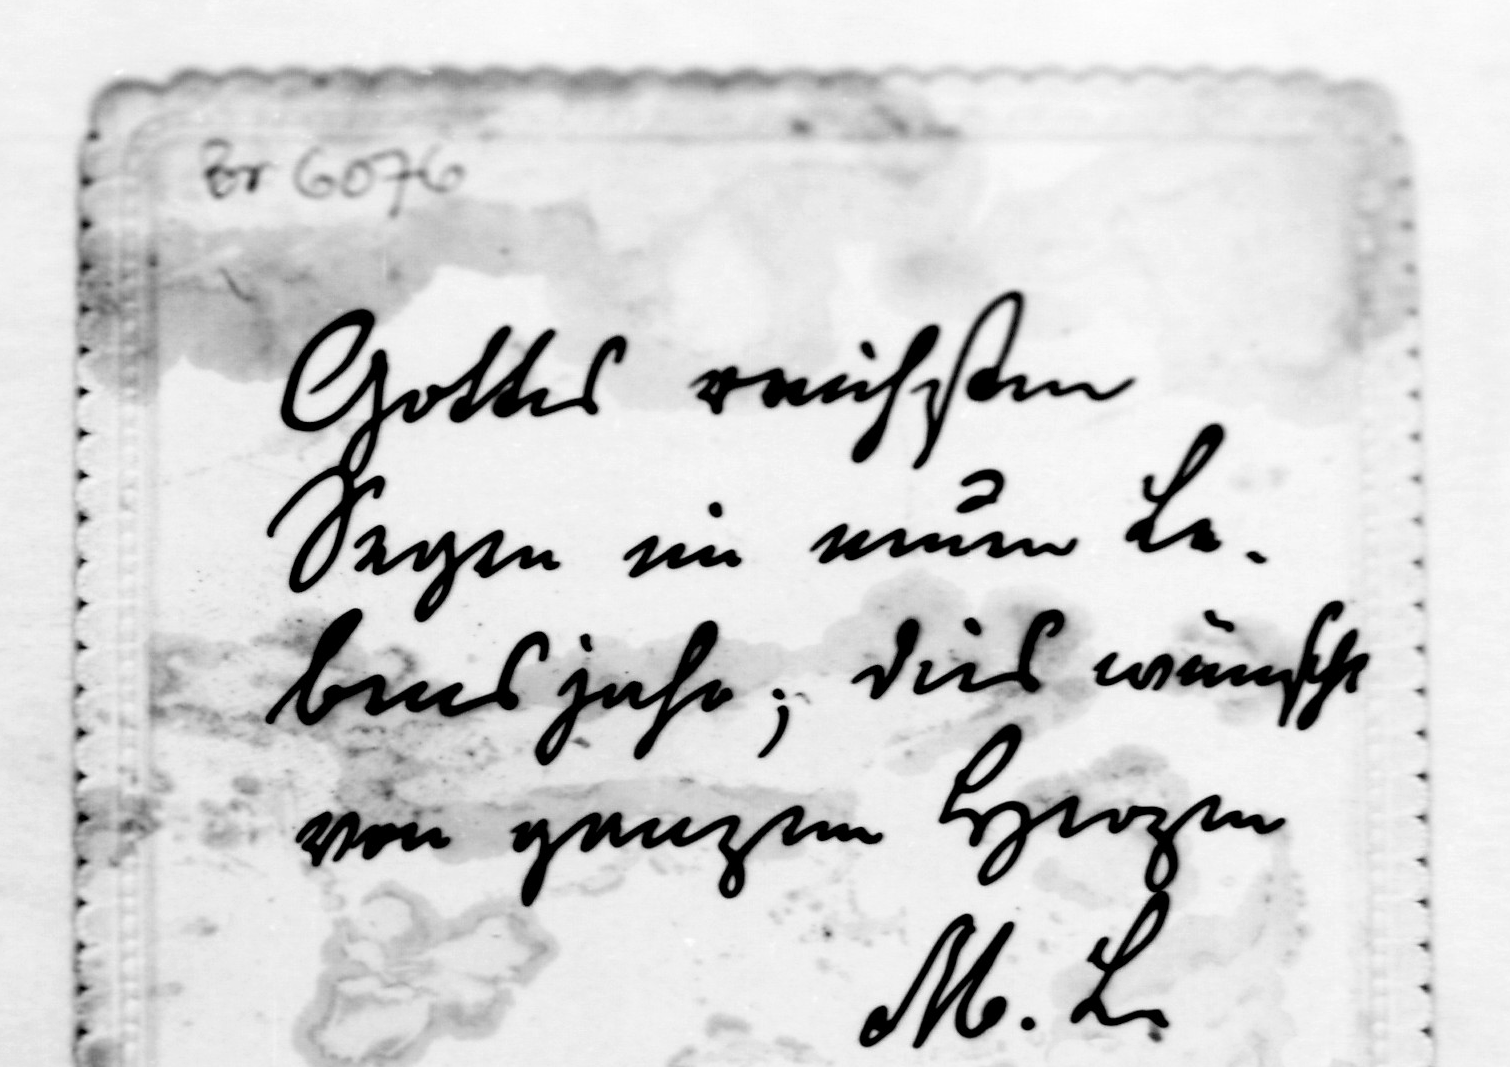
\includegraphics[width=4cm]{original.png}
%     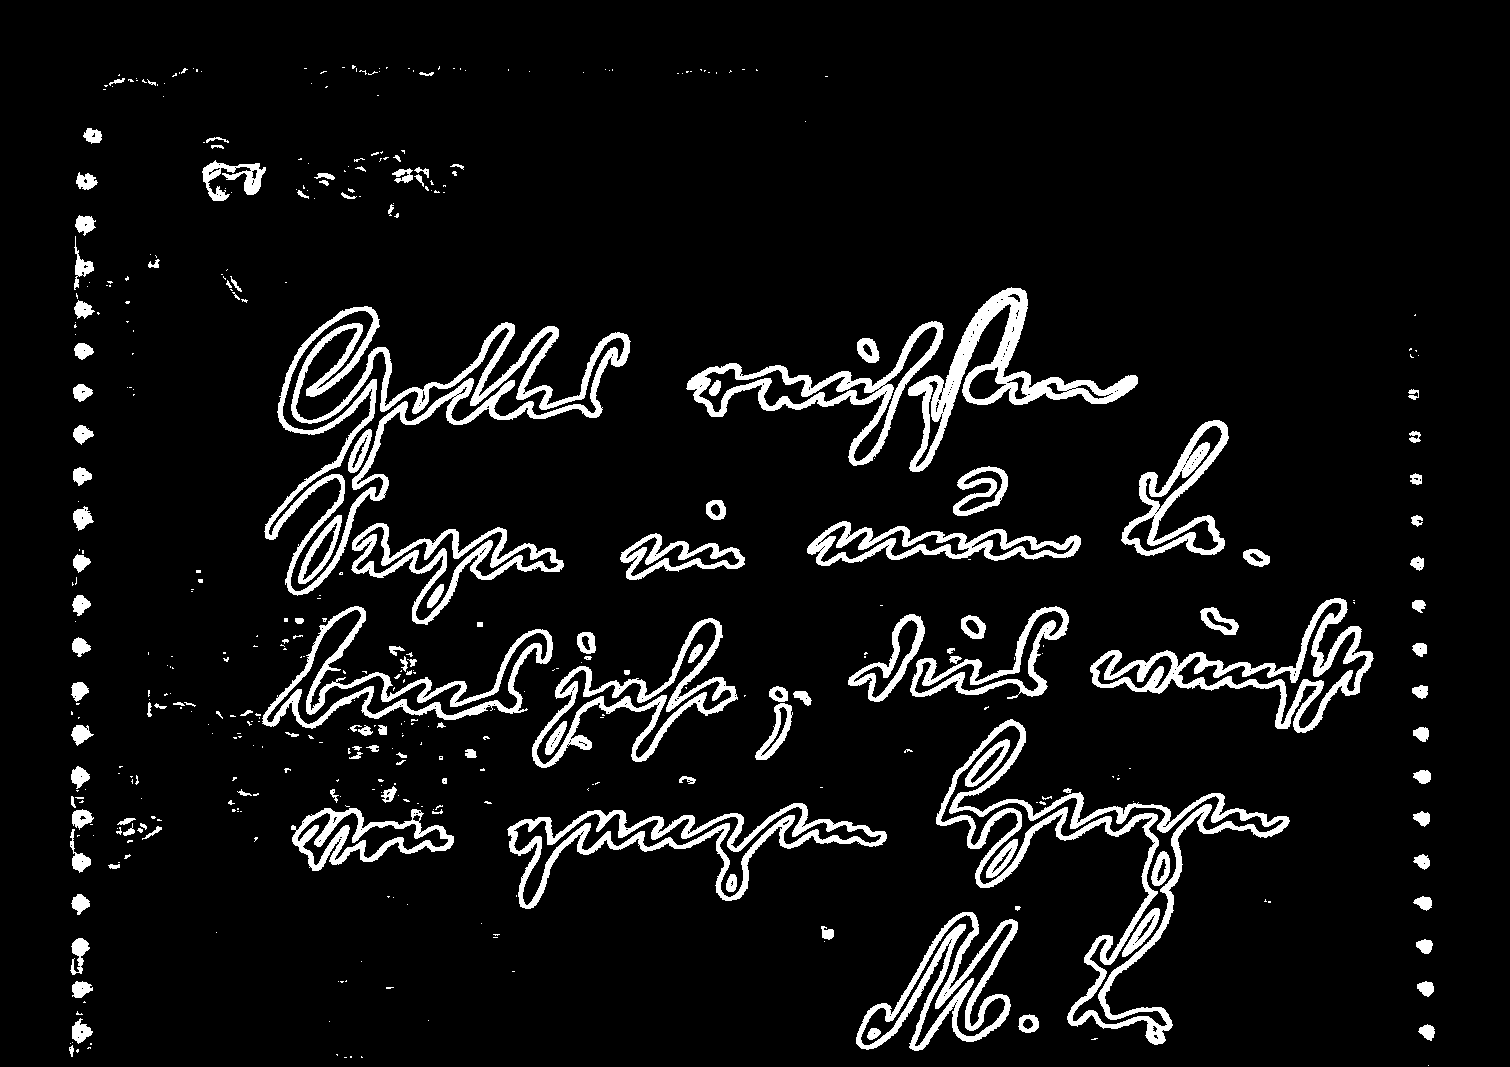
\includegraphics[width=4cm]{contrast-image.png}
%     \caption{Original Document Image and Contrast Image}
%     \label{fig:7}
% \end{figure}

% \subsection{Thresholding}

\newpage
\printbibliography
\end{document}